\documentclass{beamer}
\usetheme{Madrid}
\usepackage{amsmath, amsfonts, tikz}
\usetikzlibrary{arrows.meta, positioning, shapes.geometric}

\title[Reinforcement Learning]{Reinforcement Learning: Principles and Algorithms}
\author{Morten Hjorth-Jensen}
\institute{Preliminary notes}
\date{May, 2024}

\begin{document}

% Title Slide
\begin{frame}
 \titlepage
\end{frame}

% Outline
\begin{frame}{Outline}
 \tableofcontents
\end{frame}

\section{Introduction}
\begin{frame}{Motivation and Applications}
 \begin{itemize}
   \item RL is used in robotics, game playing (AlphaGo), finance, recommendation systems.
   \item Learn from interaction with environment.
   \item Optimal control and decision making.
 \end{itemize}
\end{frame}

\begin{frame}{What is Reinforcement Learning?}
 \begin{itemize}
   \item An area of machine learning concerned with how agents ought to take actions to maximize cumulative reward.
   \item Trial-and-error learning.
   \item Feedback is delayed and sparse.
 \end{itemize}
\end{frame}

\section{RL Framework}
\begin{frame}{Agent-Environment Interaction}
 \centering
 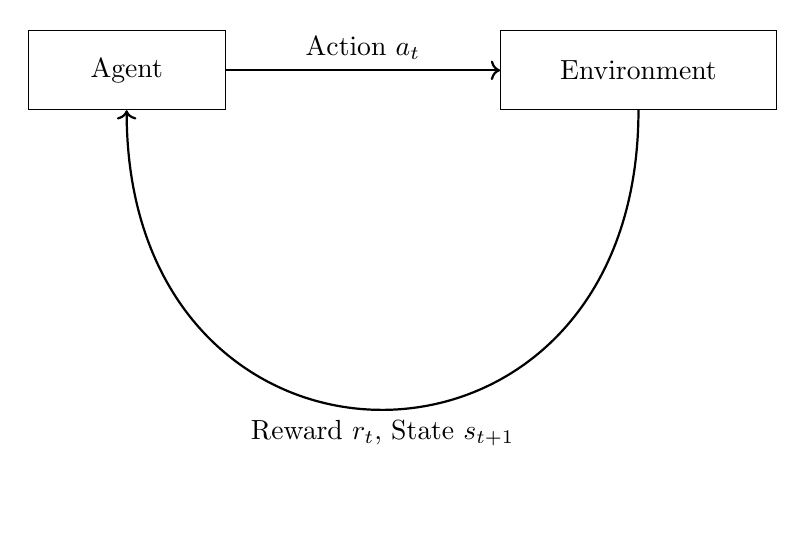
\begin{tikzpicture}[node distance=2.5cm, every node/.style={align=center}]
   \node[draw, rectangle, minimum width=2.5cm, minimum height=1cm] (agent) {Agent};
   \node[draw, rectangle, minimum width=3.5cm, minimum height=1cm, right of=agent, xshift=4cm] (env) {Environment};

   \draw[->, thick] (agent) -- node[above] {Action $a_t$} (env);
   \draw[->, thick] (env) to[out=270,in=270,looseness=2] node[below] {Reward $r_t$, State $s_{t+1}$} (agent);
 \end{tikzpicture}
\end{frame}

\begin{frame}{Markov Decision Processes (MDPs)}
 \begin{itemize}
   \item MDP is defined by $(\mathcal{S}, \mathcal{A}, P, R, \gamma)$.
   \item $\mathcal{S}$: set of states.
   \item $\mathcal{A}$: set of actions.
   \item $P(s'|s,a)$: transition probabilities.
   \item $R(s,a)$: reward function.
   \item $\gamma \in [0,1]$: discount factor.
 \end{itemize}
\end{frame}

\begin{frame}{MDP Transition Diagram (Example)}
 \centering
 \begin{tikzpicture}[->, >=stealth', shorten >=1pt, auto, node distance=3.5cm,
   thick, main node/.style={circle, draw, font=\sffamily\Large\bfseries}]

   \node[main node] (1) {$s_1$};
   \node[main node] (2) [right of=1] {$s_2$};
   \node[main node] (3) [below of=1, yshift=1cm] {$s_3$};

   \path[every node/.style={font=\sffamily\small}]
     (1) edge[bend left] node[above] {$a_1$} (2)
         edge[bend right] node[left] {$a_2$} (3)
     (2) edge[loop right] node {$a_1$} (2)
     (3) edge[bend left] node[right] {$a_1$} (1);
 \end{tikzpicture}
\end{frame}

\section{Value Functions}
\begin{frame}{Reward Signal and Return}
 \begin{itemize}
   \item Return $G_t = \sum_{k=0}^{\infty} \gamma^k r_{t+k+1}$.
   \item Objective: Maximize expected return.
   \item Reward hypothesis: All goals can be framed as the maximization of expected cumulative reward.
 \end{itemize}
\end{frame}

\begin{frame}{Value Functions}
 \begin{itemize}
   \item State-value: $V^\pi(s) = \mathbb{E}_\pi[G_t | s_t = s]$.
   \item Action-value: $Q^\pi(s,a) = \mathbb{E}_\pi[G_t | s_t = s, a_t = a]$.
 \end{itemize}
\end{frame}

\begin{frame}{Bellman Equations}
 \begin{itemize}
   \item $V^\pi(s) = \sum_a \pi(a|s) \sum_{s'} P(s'|s,a)[R(s,a) + \gamma V^\pi(s')]$.
   \item $V^*(s) = \max_a \sum_{s'} P(s'|s,a)[R(s,a) + \gamma V^*(s')]$.
 \end{itemize}
\end{frame}

\section{Learning Algorithms}
\begin{frame}{Dynamic Programming}
 \begin{itemize}
   \item Requires a model of the environment.
   \item Policy evaluation and improvement.
   \item Value iteration and policy iteration.
 \end{itemize}
\end{frame}

\begin{frame}{Monte Carlo Methods}
 \begin{itemize}
   \item No model needed.
   \item Learn from complete episodes.
   \item First-visit and every-visit MC methods.
 \end{itemize}
\end{frame}

\begin{frame}{Temporal-Difference (TD) Learning}
 \begin{itemize}
   \item Learn from incomplete episodes.
   \item TD(0): $V(s_t) \leftarrow V(s_t) + \alpha [r_{t+1} + \gamma V(s_{t+1}) - V(s_t)]$.
 \end{itemize}
\end{frame}

\begin{frame}{SARSA and Q-Learning}
 \begin{itemize}
   \item SARSA: on-policy.
   \item Q-Learning: off-policy.
   \item Both update $Q(s,a)$ from experience.
 \end{itemize}
\end{frame}

\section{Deep Reinforcement Learning}
\begin{frame}{Exploration vs Exploitation}
 \begin{itemize}
   \item Need to balance exploring new actions and exploiting known rewards.
   \item $\epsilon$-greedy strategy.
 \end{itemize}
\end{frame}

\begin{frame}{Function Approximation}
 \begin{itemize}
   \item Use neural networks to approximate $Q(s,a)$ or $\pi(a|s)$.
   \item Generalizes across states and actions.
 \end{itemize}
\end{frame}

\begin{frame}{Deep Q-Networks (DQN)}
 \begin{itemize}
   \item Neural net to approximate $Q(s,a)$.
   \item Uses experience replay and target networks.
 \end{itemize}
\end{frame}

\begin{frame}{Policy Gradient Methods}
 \begin{itemize}
   \item Directly parameterize and optimize the policy.
   \item Use gradient ascent: $\nabla_\theta J(\theta)$.
 \end{itemize}
\end{frame}

\begin{frame}{Actor-Critic Methods}
 \begin{itemize}
   \item Combine value function (critic) with policy (actor).
   \item Advantage Actor-Critic (A2C), A3C.
 \end{itemize}
\end{frame}

\begin{frame}{Advanced Algorithms}
 \begin{itemize}
   \item PPO: stable updates via clipping.
   \item SAC: maximum entropy RL.
 \end{itemize}
\end{frame}

\section{Conclusion}
\begin{frame}{Challenges in RL}
 \begin{itemize}
   \item Sample inefficiency.
   \item Exploration in sparse reward environments.
   \item Stability of training with function approximation.
 \end{itemize}
\end{frame}

\begin{frame}{Applications}
 \begin{itemize}
   \item Games: AlphaGo, StarCraft.
   \item Robotics.
   \item Healthcare, Finance.
 \end{itemize}
\end{frame}

\begin{frame}{Summary}
 \begin{itemize}
   \item RL is about learning through interaction.
   \item MDPs, value functions, policy learning are key concepts.
   \item Algorithms evolve from tabular to deep methods.
 \end{itemize}
\end{frame}


\end{document}
